
\documentclass{report}

\input{preamble}
\input{macros}
\input{letterfonts}

\title{\Huge{Economia Politica}\\Sistemi Informativi Aziendali}
\author{\huge{Caberlotto Giovanni}}
\date{}

\begin{document}

\maketitle
\newpage% or \cleardoublepage
% \pdfbookmark[<level>]{<title>}{<dest>}
\pdfbookmark[section]{\contentsname}{toc}
\tableofcontents
\pagebreak

\chapter{Economia Pubblica e le Diverse Libertà} % (fold)

\label{chap:Economia Pubblica e le Diverse Libertà}

\section{L'economia pubblica}

\subsection{L'oggetto di studio}

\dfn{Economia Pubblica}{L'economia pubblica è la branca della disciplina economica che studia le possibili forme di intervento pubblico nei sistemi economici}

In questa definizione spiccano due paroli chiave - "possibili e pubblico" - a ciascuna delle quali è opportuno dedicare una breve riflessione:
\begin{itemize}
  \item Si parla di "possibili forme di intervento pubblico" in quanto, tra tutte le forme di intervento pubblico, si considerano anche quelle che, pur non essendo state praticate nella realtà, potrebbero esserlo;
  \item L'aggettivo pubblico si riferisce a tutto ciò che attiene allo Stato, nei diversi significati che questo termine ha assunto nel tempo, e agli altri soggetti classificabili come appartenenti al settore pubblico.
\end{itemize}

Rispetto alla tradizionale classificazione tra microeconomia e macroeconomia, l'economia pubblica nasce e si sviluppa sopratutto con una impostazione microeconomica.
Ciò significa che si prendono in esame i singoli mercati, la domanda, l'offerta e tutto ciò che serve per l'analisi microeconomica.

In materia di economia pubblica si applica un analisi positiva e un analisi normativa:

\begin{itemize}
  \item Analisi positiva, tratta le conseguenze di una politica economica tramite analisi analitiche con tabelle dati e grafici;
  \item Analisi normativa, tratta le desiderabilità di una politica economica ovvero i giudizi di valore e le norme di comportamento.
\end{itemize}

Quando si parla di economia pubblica è importante dare anche la definizione di politica economica:
\dfn{Politica economica}{Con politica economica intendiamo l'insieme delle regole e delle azioni attuate dai governi per raggiungere gli obiettivi prefissati in campo economico e sociale.}
\ex{Politica economica}{Un esempio di politica economica può essere il contrasto dell'inflazione o in tempi più recenti la risoluzione dei problemi legati all'immigrazione}

\subsection{Le origini}

Alla fine del Medioevo, con l'affermazione degli stati moderni, si assiste all'organizzazione delle strutture politiche centrali e alla progressiva costituzione di un soggetto pubblico autonomo inoltre si determinarono nuovi ambiti di intervento pubblico (via via, oltre alla riscossione delle imposte, vengono istituzionalizzate la difesa, la sicurezza, la giustizia).
L'attenzione dei primi economisti - mentre l'economia inizia ad affermarsi come scienza - cade sulle nuove forme di intervento dello Stato, e in particolare sul prelievo fiscale. Per questo motivo l'economia pubblica sopratutto in Italia, si configura inizialmente come scienza delle finanze.
\dfn{Scienza delle finanze}{analizza le tre funzioni essenziali attribuite all'intervento pubblico (allocativa, redistributiva e di stabilizzazione macroeconomica) in uno specifico contesto istituzionale nei sistemi capitalistici.}

Successivamente con l'avvento delle moderne costituzioni dopo la Seconda guerra mondiale lo stato iniziò ad intervenire in misura maggiore e quindi si determinò la crescita dei servizi offerti alla collettività, perciò l'economia pubblica assunse il ruolo di economia di benessere.

\section{Libertà individuali e vincoli collettivi}
\subsection{Libertà negativa e libertà positiva}

Nel linguaggio della scienza politica il termine "libertà" ha assunto due principali significati, ciascuno dei quali fa capo a due diverse forme di libertà, rispettivamente denominate libertà negativa e libertà positiva:

\dfn{Libertà Negativa}{è propria della persona che può agire senza impedimenti da parte di altri soggetti o della persona che è ciò che desidera essere. Significa assenza di impedimenti o costruzioni esterne. La libertà negativa è come la “libertà da”. Sono tutti quei diritti inviolabili delle persone, ad esempio, il diritto alla vita. Lo Stato in questa libertà può intervenire solamente in alcune situazioni (arresto).}
\cor{libertà negative}{Le libertà negative sono quelle liberta inviolabili come ad esempio il diritto all'esistenza dove lo stato può intervenire solo in occasioni estreme come l'arresto}

\dfn{Libertà Positiva}{si tratta di libertà riconosciuta ai cittadini ma rispetto alle quali lo Stato agisce concretamente. Si esprime nell'autonomia e nella autodeterminazione con cui non individuo orienta la propria volontà e le proprie azioni verso uno scopo. Autonomia nel voler ciò che si vuole e presenza delle condizioni per perseguire ciò che si vuole. La libertà positiva è come la “libertà di”. Esempio diritto al lavoro.}
\cor{Libertà positive}{Per ‛libertà positiva' s'intende nel linguaggio politico la situazione in cui un soggetto ha la possibilità di orientare il proprio volere verso uno scopo, di prendere delle decisioni, senza essere determinato dal volere altrui.}

\subsection{Liberalismo o economia sociale di mercato}

La distinzione tra libertà negative e libertà positiva può apparire astratta, essa ha importanti implicazioni di politica economica, sopratutto con riferimento ai rapporti:

\begin{itemize}
  \item tra libertà di scelta individuale e il funzionamento del mercato;
  \item tra lo Stato e il mercato.
\end{itemize}

Considera la libertà negativa "libertà da" essa può essere intesa come libertà sopratutto dal potere politico (ovvero dallo Stato).

\ex{}{Pensiamo agli Stati Uniti d'America, un paese ritenuto la patria del liberalismo. Lo stato Impone ai cittadini una tassazione che, mediamente è più bassa di molti altri Paesi (per esempio quelli Europei). In questo modo lascia ai cittadini maggiori risorse a disposizione. Dall'altro lato però, lo Stato fa sì che siano i cittadini stessi a dover finanziare buona parte delle loro spese sanitarie per esemio, stipulando delle polizze di assicurazione private, della previdenza e anche delle spese per l'istruzione dei giovani.}

La libertà positiva "libertà di", invece, corrisponde alla libertà delle persone di realizzare i propri obiettivi e attiene quindi alle loro effettive opportunità di scelta.

\ex{}{Sappiamo che le scelte di acquisto di un cittadino sono limitate dal suo vincolo di bilancio, ossia dalle risorse a sua disposizione. L'assenza di reddito, per esempio in conseguenza di una prolungata disoccupazione, impedisce di acquistare i beni desiderati o addirittura neccesari. Contrastando efficacemente la disoccupazione o fornendo un sostegno economico ai disoccupati, lo Stato può favorire una importante libertà positiva, ovvero la libertà di condurre una vita dignitosa.}

In ambito economico, coloro che sostengono la prevalenza della libertà negativa sulla libertà positiva privilegiano l'assenza di costrizioni e vincoli, da parte sopratutto dello Stato, e la cosidetta libertà di mercato. questa imposizione deriva dalla teoria politica del liberismo.

\dfn{Liberismo}{Secondo i liberisti lo Stato deve limitarsi a svolgere soltanto alcune funzioni essenziali di controllo, evitando di esercitare il potere coercitivo in ambito economico}

\nt{Con potere coercitivo intendiamo il potere di costringere}
In tempi moderni si è sviluppato una nuova tipologia di Stato analoga allo stato liberale:
\dfn{Stato minimale}{Talvolta si parla di Stato minimale per riferirsi ai casi in cui lo Stato si limita ad assicurare quei servizi come giustizia difesa e sicurezza e quelle infrastrutture che il mercato non sarebbe in grado di mettere a disposizione in modo adeguato, data la loro natura di beni pubblici}
è importante quindi definire il termine bene pubblico.

\dfn{Beni pubblici}{Con beni pubblici intendiamo i beni per i quali non vi è rivalità nel consumo e vi è non escludibilità dal consumo}

Da quanto citato in precedenza è facile dedurre che più lo stato è minimale altrettanto sarà minima la tassazzione imposta ai cittadini. 

I sostenitori della libertà positivà al contrario, rivendicano uno Stato con un ruolo più esteso nelle politiche economiche e sociali; Secondo essi lo Stato dovrebbe anche rimuovere gli ostacoli che limitano la "libertà di", Quando l'intervento economico dello Stato risponde a queste neccessità si parla di economia sociale di mercato.

Molti Paesi occidentali hanno declinato le numerose versioni di questo modello, collocandosi per così dire a metà strada tra Stato minimale e Stato pianificatore.
\nt{Il modello più completo di economia sociale è il modello scandinavo}

\chapter{L'intervento pubblico: finalità e modalità} % (fold)
\label{chap:L'intervento pubblico: finalità e modalità}

\section{Le finalità dell'intervento pubblico}

Nell'1958 l'economista americano Richard Musgreve (1910-2007) propose una classificazione - ancora oggi ritenuta valida - che spiega le diverse forme di intervento pubblico in base alle tre principali finalità che potevano ispirarle:

\begin{itemize}
  \item Finalità allocativa;
  \item Finalità redistributiva;
  \item Finalità di stabilizzazione e crescità.
\end{itemize}

\subsection{Finalità allocativa}
\dfn{Finalita allocativa}{Con finalità allocativa intendiamo la finalità perseguita dall'operatore pubblico che intende migliorare il funzionamento dei mercati.}

La finalità allocativa cerca di destinare le risorse nel modo più efficente possibile.
Le risorse economiche vanno allocate nel modo più ottimale possibile per il raggiungimento del benessere collettivo.

\subsubsection{I fallimenti del mercato}

Le motivazioni secondo cui lo Stato interviene in economia sono correlate ai fallimenti del mercato.

\dfn{Fallimenti del mercato}{Si dicono fallimenti del mercato le situazioni in cui il mercato non consente una ottimale allocazione delle risorse, e presenta dunque margini di miglioramento in termini di efficenza e di incrementi di benessere}

i fallimenti del mercato sono:

\begin{itemize}
  \item Monopolo;
  \item Assimetrie informative;
  \item Esternalità negative;
  \item Beni pubblici e beni meritori
\end{itemize}

\subsubsection{Monopoli}

Sono fallimenti del mercato per esempio la presenza di monopoli, L'impresa monopolitica non rispetta la legge di determinazione di domanda e offerta in quanto è l'unica operatrice nel settore. una forma di intervento viene addottata istituendo monopoli pubblici o con legislazioni antitrust

\subsubsection{Assimetrie informative}

Un altro esempio di fallimento del mercato sono le asimmetrie informative esistenti tra gli acquirenti e venditori quando una delle due parti (di solito il venditore) dispone di maggiori informazioni rispetto all'altra. Il mercato fallisce perché non importa vantaggi reciproci ai soggetti coinvolti.
Spesso ciò avviene con le banche. 
 La normativa bancaria informativa è molto dettagliata e quindi per una persona comune non addentrato nel settore è un rischio stipulare determinati contratti e svolgere certe operazioni. In questo caso la normativa impone degli obblighi rigorosi. Questa rigorosità viene esercitata con la banca che deve avere una serie di obblighi e comportamenti volti a tutela del cliente.

 \subsubsection{Esternalità negative}

La presenza di esternalità, soprattutto negative, conduce a equilibri di mercato inefficienti perché il prezzo del bene non tiene conto dei costi sociali derivanti dalla produzione. 

\ex{Una catena della grande distribuzione decide di realizzare un nuovo centro commerciale in una determinata zona. Questa scelta può compromettere il benessere dei residenti di quella zona per via dell'inquinamento acustico o della congestione del traffico. solo lo stato può costringere le aziende a farsi carico dei costi sociali dell'inquinamento e degli altri disagi subiti dalla collettività. Generalmente con incentivi/discentivi di natura fiscale o con una legislazione del tipo command and control}

\nt{Dalla produzione deriva principalmente il fenomeno dell’inquinamento. La normativa interviene attraverso delle sanzioni. Ad esempio, per coloro che non rispettano la normativa sulla sicurezza, sugli inquinamenti. Interviene con delle agevolazioni economiche per le imprese che adottino delle apparecchiature che tendano a ridurre l’impatto della produzione sull’ambiente. }

\subsubsection{Beni pubblici e beni meritori}

Lo stato produce beni che gli imprenditori privati non produrrebbero E' importnte distinguere tra beni pubblici e beni meritori:

\dfn{Beni pubblici}{sono quei beni che lo Stato fornisce gratuitamente o quasi ai cittadini perché ritiene che soddisfino un superiore interesse della collettività.}

\dfn{Beni Meritori}{sono quei beni che, oltre a soddisfare un bisogno individuale generano esternalità positive, favorendo lo sviluppo morale e sociale di tutta la collettività. Sono beni che possono essere prodotti anche dal libero mercato ma che lo Stato ritiene debbano essere prodotti e consumati in misura superiore alla loro domanda effettiva.}

\nt{La produzione di entrambe le tipologie di beni elencate è attribuita allo Stato nell'interesse della collettività.}


\subsection{La finalità redistributiva}

Gli scambi di mercato contribuiscono a determinare una certa distribuzione del reddito e della ricchezza. 
Le condizioni di partenza di un soggetto sono rilevanti ai fini del risultato finale. Il successo economico e sociale di un individuo dipende dal suo impegno nel raggiungere gli obiettivi. Esistono vantaggi e svantaggi che poco hanno a che fare con l’impegno. Tutto questo può portare ad una distribuzione delle risorse molto disuguale mentre molti soggetti si trovano in condizioni di indigenza.

\ex{Chi nasce e cresce in una famiglia colta e benestante ha a disposizione occasioni di studio e di arricchimento personale sicuramente maggiori rispetto a coloro che nascono in realtà familiari più modeste. tale disuguaglianza nelle condizioni di partenza è evidente anche a livello globale: nascere e crescere in un paese povero e flagellato da guerre e carestie non offre le stesse opportunità che nascere e crescere in un quartiere benestante di una città occidentale.}

\dfn{Finalità redistributiva}{Con finalità redistributiva si intende la finalità perseguita dall’operatore pubblico che intende ridurre le disparità tra le persone, generate dal mercato o da circostanze esterne e considerate ingiuste. L’operatore pubblico tende a ridurre le disuguaglianze rispetto a risorse e opportunità che ciascun individuo ha a disposizione. È ispirata dal concetto di uguaglianza, inteso come uguali opportunità offerte a tutti e quindi dal concetto di equità, inteso come uguale trattamento di uguali e diverso trattamento di individui disuguali.}

Lo strumento principale con cui lo Stato mette in atto il suo obiettivo di equità è la politica fiscale, composta di tassazione e spesa pubblica. Con essa lo Stato cerca di riequilibrare la distribuzione delle risorse a favore di coloro che si trovano sugli scalini inferiori della scala dei redditi e delle opportunità.

\nt{Politica fiscale significa ricorrere alle imposte, alla spesa pubblica}

\ex{Se lo Stato aumentasse la tassazione sui redditi più alti, potrebbe disporre di risorse da redistribuire ai cittadini meno abbienti, magari aumentando il livello delle pensioni minime oppure riducendo le tasse universitarie agli studenti appartenente a famiglie con redditi modesti.}

\nt{Ci sono numerose indagini che fotografano i redditi delle famiglie italiane negli ultimi 10 anni e confermano un netto aumento delle disuguaglianze economiche.}

\subsection{Finalità di stabilizzazione}

I sistemi economici sono caratterizzati da andamento ciclici in cui si alternano fasi di forte intensità e fasi di bassa intensità.
La crisi bancaria del 2008 è stata seguita da una stagione di recessione e poi da una lunga di sostanziale stagnazione che in molti Paesi non si era ancora conclusa nel 2020. 
Che si tratti di (PIL cala) o di (PIL cresce poco) i Governi provano a far ripartire l’economia attraverso gli strumenti a loro disposizione su scala macroeconomica, a cominciare dalle politiche fiscali e monetarie. 
L’intervento pubblico è necessario quando l’economia corre troppo per evitare che si raggiungono picchi di domanda troppo elevati con conseguente inflazione. 

\dfn{Finalità di stabilizzazione}{è la finalità perseguita dall’operatore pubblico che intente “stabilizzare” il sistema economico contrastando gli effetti delle fasi negative dei cicli economici, spingendo nella direzione del pieno impiego e di un’inflazione sotto controllo.}

\nt{è la terza finalità dello Stato. Si tratta di una finalità diretta a far crescere l’economia attraverso l’utilizzo della politica fiscale monetaria. Attraverso ad essa, è possibile contrastare l’inflazione.}

\subsection{Finalità e strumenti}

Le tre finlità sono perseguite con modalità differenti:
\begin{itemize}
  \item Finalità allocativa:  richiede l’impegno di strumenti prevalentemente microeconomici, volti a correggere i fallimenti di specifici mercati;
  \item Finalità redistributiva 
viene perseguita attraverso la politica fiscale, riassunta dal bilancio dello Stato. Essa si compone di strumenti sia macroeconomici sia microeconomici; 
  \item Finalità di stabilizzazione richiede l’utilizzo di strumenti prevalentemente macroeconomici in grado di agire sui consumi totali, gli investimenti complessivi e sul PIL e sull’occupazione.
\end{itemize}

Sarebbe ingenuo tentare di stabilire una corrispondenza biunivoca tra le poche finalità e i tanti strumenti a disposizione dello Stato per intervenire nel sistema economico.

\subsection{Finalità dell'intervento statale e spesa pubblica nell'epoca contemporanea}

Nell’800 si riteneva che l’unica finalità economica che giustificasse l'intervento degli Stati nazionali fosse quella allocativa, che era rivolta alla difesa di alcuni diritti individuali. I quali prevedevano un'impostazione liberale rivolta alla tutela delle libertà negative e a sostegno dello Stato minimale. Le risorse ricavate dall'imposizione fiscale venivano impiegate dai governi per il mantenimento dell'apparato burocratico e per pochi altri scopi.
Nel 1870 la spesa pubblica nei paesi industrializzati era in media attorno all'8\% Del PIL.
Verso la fine del diciannovesimo secolo l'affermazione della rivoluzione industriale pone allo stato nuovi problemi, legati all'organizzazione e alla crescita del proletariato. 
A partire dalla Germania la finalità redistributiva comincia a far parte delle finalità dell'azione pubblica.
Fino alla Prima guerra mondiale, l'impostazione liberale continua prevalere e il peso dello Stato sul PIL non subisce variazioni di rilievo.
Il finanziamento della spesa militare per il primo conflitto mondiale richiede un deciso aumento dell'imposizione fiscale.
I due conflitti mondiali causarono milioni di morte immani distruzioni, e sollecitarono l'intervento attivo dello Stato nella ricostruzione post bellica e nel sostegno alle famiglie colpite da lutti e menomazioni fisiche.
L'aumento della spesa pubblica è imputabile agli incrementi della spesa sociale, resi necessari dalla grande depressione degli anni 30 del secolo scorso.
Negli Stati Uniti per contrastare la disoccupazione di massa e rilanciare l'economia lo stato interviene attuando il NEW DEAL ideato da Franklin Delano Roosevelt. Esso prevedeva una imponente serie di investimenti nella costruzione di opere pubbliche e nell'erogazione di sussidi per i disoccupati e per le persone più bisognose. La finalità di stabilizzazione si aggiunge alle altre due finalità dell'intervento pubblico.
Nel 1960 la spesa pubblica raggiunge quasi il 30\% del PIL.
Dallo stato minimale dei liberali ottocenteschi si è passati all'economia sociale di mercato.
Nel periodo del 1960-1980 si registra il più marcato incremento di spesa pubblica rilevato in periodo di pace.
Nelle costituzioni approvate dopo la seconda guerra mondiale diventavano centrali alcune libertà positive sotto forma di diritti:

\begin{itemize}
  \item Diritto al lavoro;
  \item Diritto all'istruzione;
  \item Diritto alla salute;
  \item Diritto all'esistenza.
\end{itemize}
a partire dagli anni 70 cominciarono a manifestarsi seri dubbi Sull'efficacia della spesa pubblica, al punto che l'elezione di Ronald Reagan Negli Stati Uniti e di Margeret Thatcher in Gran Bretagna porta il governo un'impostazione neoliberista, detta economia dell'offerta (supply – side economics). 
Si tratta di un'impostazione macroeconomica che si pone in aperto contrasto con le teorie keynesiane che sostengono la spesa pubblica.
Lo strumento principale della supply-side economics e la politica fiscale sui redditi da lavoro, basata sul modello della curva di Laffer. Secondo questo modello mantenendo basso il livello di tassazione sui redditi l'offerta di lavoro tenderebbe ad aumentare e anche la produzione e la crescita economica. 
L'impostazione neoliberista ha dominato le politiche economiche di molti paesi per circa un quarto di secolo. Essa era volta a ridurre lo spazio di azione dell'intervento pubblico attraverso politiche di privatizzazione e deregolamentazione dei mercati.
I risultati deludenti non hanno interrotto le tendenze precedenti e il peso della spesa pubblica sul PIL raggiunge mediamente il 45\%.
\nt{lo Stato dell’800, quello che applica il modello neoliberista, è caratterizzato dall’esercizio di una funzione allocativa. La funzione redistributiva e di stabilizzazione sono proprie dello Stato che adotta un modello sociale e democratico.}
La spesa pubblica progressivamente, dalla rivoluzione industriale ad oggi, ha continuato ad aumentare. L’aumento è dovuto dal fenomeno della rivoluzione industriale. Con essa si è costituita la classe di proletariato. Gli abitanti si sono spostati dalle campagne alle città. Gli abitanti delle città hanno iniziato a chiedere una serie di servizi. Richiedere servizi, cioè aumentare l’intervento dello Stato in economia, aumentando il prelievo fiscale e aumentando la spesa pubblica. Nel XIX secolo inizia ad essere utilizzata la finalità redistributiva affiancata alla finalità allocativa. 

La curva di laffer mette in relazione il gettito fiscale dell'imposta sui redditi e l'aliquota fiscale.
Secondo l'economista americano e i suoi seguaci questa relazione può essere rappresentata graficamente con la forma di una U rovesciata. Alzando l'aliquota il gettito inizialmente aumenterebbe; se l'aliquota salisse oltre un certo livello, il gettito inizierebbe a calare.
Ciò significa che i soggetti economici sarebbero disincentivati a lavorare e a produrre, provocando ripercussioni negative sulla crescita economica.

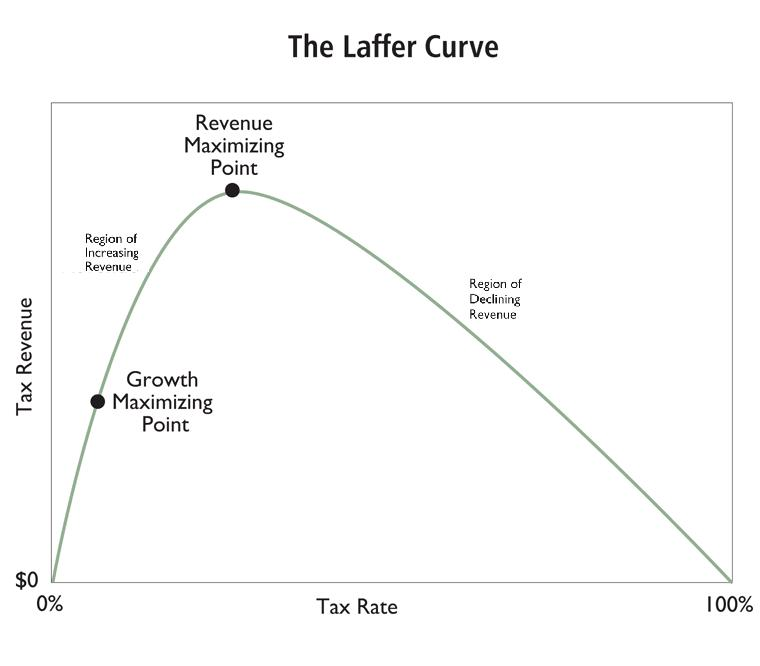
\includegraphics[width=0.6\textwidth]{./graphs/laffer-curve.jpg}

\subsection{La rivincita dello stato}
gli ultimi due decenni del secolo scorso e l'inizio di quello attuale sono stati caratterizzati da un'impostazione neoliberista.
Questa impostazione ha circoscritto la presenza pubblica nell'economia, ha ridotto la tassazione sulle imprese e sui redditi più elevati dei contribuenti e ha limitato l'estensione del welfare state anche in ambiti come l'istruzione e la sanità.
Due episodi hanno scosso le economie mondiali è incrinato la fiducia nella capacità di ai mercati di stabilizzarsi da soli.
\begin{itemize}
  \item Il primo è stato il fallimento della banca americana il 15 settembre 2008 e la successiva crisi finanziaria;
  \item Il secondo all'inizio del 2020, e la crisi economica innescata dalla pandemia COVID-19
\end{itemize}
Entrambi i casi, l'intervento degli Stati ha costituito l'unica soluzione per contenere le gravissime conseguenze sulle popolazioni.

La crisi finanziaria nel 2008 è stata contrastata dall'intervento pubblico di salvataggio delle banche e di sostegno a famiglie e imprese.

\nt{la crisi del 2008, successivamente la pandemia e oggi la guerra hanno portato alla rivalutazione dell’intervento dello Stato in economia.}

\section{Le politiche macroeconomiche} % (fold)
\label{sec:Le politiche macroeconomiche}
\subsection{Le politiche economiche e la loro classificazione}
\dfn{Politica Economica}{La politica economica è l'insieme degli interventi pubblici (dello stato e di altre amministrazioni pubbliche) finalizzati a modificare una o più variabili del sistema economico. Ciascuno di essi opera in modo assai diverso sulle condizioni economiche di una popolazione}
\\
Possiamo individuare una prima classificazione tra politiche macroeconomiche e politiche microeconomiche.
Le prime si rivolgono all'intero sistema economico e si dividono in politiche monetarie e politiche fiscali, le seconde sono rivolte a uno specifico settore produttivo o a uno specifico territorio
\\
\begin{table}[h]
    \centering
    \begin{tabular}{|l|l|l|}
        \hline
        Campo & \textbf{Microeconomia} & \textbf{Macroeconomia} \\
        \hline
        Oggetto di Studio & Comportamento Economico & Comportamento Economico \\
                           &                         & Intero sistema economico \\
        \hline
        Livello dell'Analisi & Decisioni dei singoli agenti economici & Intero sistema economico \\
        \hline
        Variabili Studiate & \begin{tabular}[c]{@{}l@{}}- Decisioni dei singoli agenti economici\\ (famiglie, consumatori e imprese)\end{tabular} & - Interi sistema economico \\
                           & - Relazioni tra imprese e consumatori & \begin{tabular}[c]{@{}l@{}}- Trend e fluttuazioni dell'attività\\ economica complessiva di un Paese o\\ di più Paesi\end{tabular} \\
                           & - Ammontare della produzione di un'impresa o\\ del reddito di un consumatore & - Relazioni tra le grandezze aggregate \\
                           & - Quantità domandate e offerte di alcuni beni & - Determinazione dei prezzi assoluti \\
                           & - Prezzi relativi & \\
        \hline
        Problemi Studiati & \begin{tabular}[c]{@{}l@{}}- Condizioni per l'allocazione\\ efficiente delle risorse\end{tabular} & \begin{tabular}[c]{@{}l@{}}- Riequilibrio e sviluppo territoriale,\\ Tutela della concorrenza e sorveglianza\\ di mercati monopolistici\end{tabular} \\
                           & - Determinazione dei prezzi relativi & \begin{tabular}[c]{@{}l@{}}- Promozione di settori industriali o\\ di ricerca e sviluppo, Occupazione di\\ categorie deboli\end{tabular} \\
        \hline
        Obiettivi delle Politiche Economiche & - Efficienza & \begin{tabular}[c]{@{}l@{}}- Politica fiscale, Politica monetaria,\\ Politiche di bilancio, Politica dal lato\\ dell'offerta, Politica dei tassi di cambio,\\ Investimenti infrastrutturali, Stabilizzazione\end{tabular} \\
                           & - Equità & \\
        \hline
        Tipi di Politiche Economiche & \begin{tabular}[c]{@{}l@{}}- Investimenti sociali e politiche del\\ lavoro, Politiche industriali, Politiche\\ della concorrenza, Politiche fiscali\end{tabular} & \\
        \hline
    \end{tabular}
    \caption{Descrizione di Microeconomia e Macroeconomia}
    \label{tab:macro_micro_economics}
\end{table}
\\
\subsection{La politica monetaria}
\dfn{Politica Monetaria}{La politica monetaria è l'insieme degli interventi volti ad aumentare o diminuire l'offerta di moneta in circolazione, attuati per modificare le condizioni del mercato monetario e con esse le dinamiche del sistema economico}
\\
La politica monetaria è gestita dalla Banca Centrale dei singoli Stati, nei paesi dell'eurozona è gestita dalla BCE il quale compito prioritario è assicurare la stabilità dei prezzi, più precisamente, essa opera perchè il tasso di inflazione nell'area dell euro non si discosti dall' 2\% annuo.
% section Le politiche macroeconomiche (end)

\end{document}

